%!TEX program = xelatex
% 完整编译: xelatex -> bibtex -> xelatex -> xelatex

\documentclass[lang=cn,11pt,a4paper]{elegantpaper}
\usepackage{float}
%\title{本次报告仅讲述综合设计部分内容}



%\institute{实验10:综合实验}
%\author{林成渊 \\ PB18051113}


%\version{0.08}
%\date{\zhtoday}

\begin{document}

\begin{center} 
	\zihao{1} 中国科学技术大学计算机学院\\
	\zihao{1} 《数字电路实验》报告\\
	\ \\
%\end{center}

\begin{figure}[H]
	\centering
	
\includegraphics[width=300pt]{logo.png}
\end{figure}

%\begin{center} 
	\zihao{2} \ \\
			  实验题目:综合实验\\
			  学生姓名:林成渊\\
			  学生学号:PB18051113\\
			  完成日期:2019.12.20\\
			  \ \\
	\zihao{4} 计算机实验教学中心制\\
			  2019年09月
	
\end{center}

\begin{center}
	本次报告仅讲述综合设计部分内容
\end{center}

\section{实验目的}

\begin{itemize}
	\item 熟练掌握前面实验中的所有知识点
	\item 熟悉几种常用通信接口的工作原理及使用 
	\item 独立完成具有一定规模的功能电路设计
\end{itemize}

\section{实验环境}

\begin{itemize}
	\item 搭载Win10系统的个人电脑
	\item 编辑器(Notepad++)
	\item Vivado2019.1
	\item vlab.ustc.edu.cn平台
	\item FPGA 实验平台(Nexys4 DDR)
	\item VGA显示器
\end{itemize}

\section{设计思路与核心框架}

整个设计分为三个主要部分,分别为文本编辑器部分、编译部分、执行部分。三个部分功能串联实现我们需要的结果。通过一个统一的时序安排电路来编排三个部分的功能执行。

\subsection{文本编辑器}

由于缺乏合适的键盘,思路是设计一套简化版的八位字符编码,利用开发板上的八位SW表示编码,按动按键input进行字符与字符间的串行输入。

\begin{figure}[H]
	\centering
	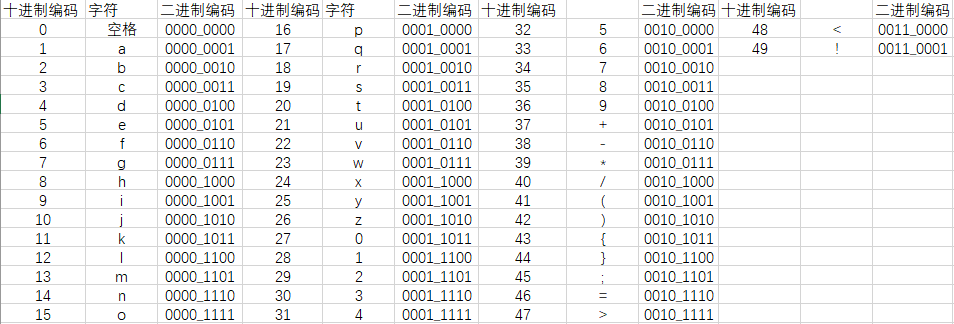
\includegraphics[width=\textwidth]{codelist.png}
	\caption{简化版八位字符编码表}
\end{figure}

随后较为关键的是与显示器的连接部分。我在显示屏上划定了一块640*640的区域,以一个英文字符8*16的占位将其分割为3200份。为此需要搭建一个Dual Port RAM,双读接口一个用于VGA接口,另一个用于编译,而SW与input通过写接口来输入文字。文字在RAM中以每个字符8位根据编码表进行存储。

\begin{figure}[H]
	\centering
	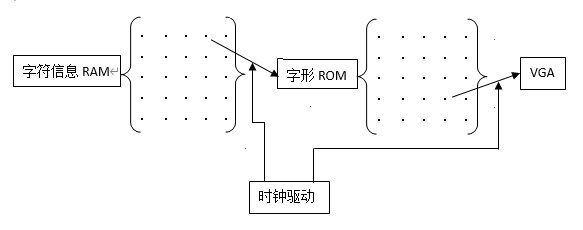
\includegraphics[width=\textwidth]{p1.png}
	\caption{文本编辑器中的显示部分}
\end{figure}

VGA接口的部分,则按照时序以一定顺序读RAM中存储的字符编码,同时通过一个预先写好的ROM将编码转为字形编码,再由VGA接口的扫描信号来依次扫描字形编码中特定位置的信息赋予输出的rgb,data。

之后需要处理的便是文本的编辑功能,这里需要引入一个光标的结构,它时刻定位在下一个字符将要输入的地址。每次写操作都以它作为基准。同时为了编辑的便捷需要,设置了回退按钮,每次按动,光标将后退一位,然后清空这一位已经写下的信息。

如此一来,一些需要顺序执行的操作,会受到Verilog中同一时刻几个操作完全并行的影响。一个通用解决办法是引入一个小型循环计数器来使各种操作严格按照先后顺序进行,不过由于涉及变量和操作较少,我采用了对于输入和退格信号分别取上下边沿的技巧,使其刚好能在一个时间周期内有序完成。

\textbf{取下边沿的模块代码}
\begin{lstlisting}
module signal_dedge(clk,button,button_rdedge);
    input clk;
    input button;
    output button_rdedge;
    reg button_r1;

always@(posedge clk)
    button_r1 <= button;
assign button_rdedge = ~button & (button_r1);
endmodule
\end{lstlisting}

\textbf{文本输入的控制代码}

\begin{lstlisting}
always @(posedge clk_65m)
begin
    if(rst)
    begin
        R_ram_we <= 0;
        R_ram_waddr <= 0;
        R_ram_wdata <= 0;
    end
    else if(backspace_redge)
    begin
        R_ram_waddr <= R_ram_waddr - 1 ;
    end
    else if(backspace_clean)
    begin
        R_ram_we <= 1;
        R_ram_wdata <= 0;
    end
    else
    begin
        if(button_rdedge)R_ram_waddr <= R_ram_waddr + 1;
        if (button_clean)
        begin
            R_ram_we <= 1;
            R_ram_wdata <= SW;
        end
        else
            R_ram_we <= 0; 
    end
end
\end{lstlisting}

\subsection{执行器}

在解释编译器之前,需要先说明执行器的结构以及“程序”的形式。我将所有的操作总结为针对指定地址内存储信息的一种操作。考虑到循环与条件判断结构的实现,由于时间原因,我采用了一个较为简化的模型,它是一个队列的存储结构(在Verilog中使用Distributed Memory的IP核实现,本质上是一个Dual Port Ram),其中每一个地址存储了一定的操作信息。

程序由R驱动按照其规定的顺序进行执行,这完成了循环的结构,同时E始终伴随条件判断语句的前后,这完成了条件判断的结构。本程序中暂时不允许循环与条件判断语句的随意嵌套,但其编写形式可以灵活地拓展为允许嵌套的结构,具体只需将条件判断的信息域外移构造一个栈,进行相应的接口对准即可,时间原因暂时只做非嵌套的版本。

如下图,每一个结点包含64bit信息。具体实现由于各操作间的先后层次明显,使用了一个循环计数器用于使各个操作有序化,效果显著。程序结束的标记设置为直接将它的下一结点引至最后的结点(第256个结点),读到该结点时结束程序。程序执行到最后会直接通过R将它导向END NODE结点,即程序队列中的最后一个结点。在那里执行的是程序的停止。除此之外,程序的每一个结点都会根据R的条件判断以将程序的下一步定位在一个特定的位置。没有循环的情况下,设定两个选择都指向下一个结点。

\begin{figure}[H]
	\centering
	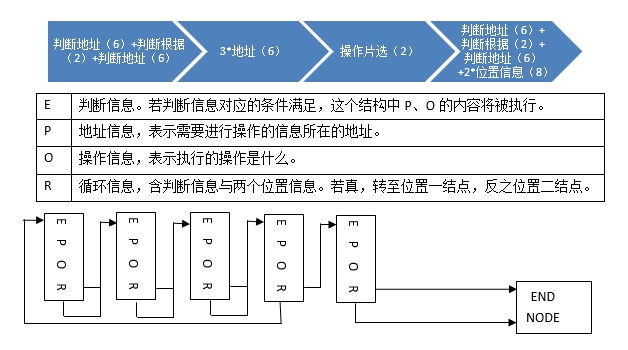
\includegraphics[width=\textwidth]{p2.png}
	\caption{程序的架构与执行流程图}
\end{figure}

所有变量的信息,与常量0-9一起存储在一个变量表里,由于信息量少,直接使用reg进行架构,变量表支持随机读取,每4bit一个信息。实际执行程序时,根据地址信息依次对每个bit的信息进行操作再拼接起来(Verilog似乎并不支持我直接利用一个变地址一次读入超1个位长的信息)。

\begin{lstlisting}
    reg [2:0]QueueNode_cnt;//循环计数量
    reg [3:0]QueueNode_a,QueueNode_b;//条件判断中转量
    reg ending;//结束信号
    reg QueueNode_E,QueueNode_R;//条件判断与循环信号
always @(posedge clk)
begin
    //为常量赋初值
    if(Queue_begin)
    begin
        Val[107:104] <= 0;
        Val[111:108] <= 1;
        Val[115:112] <= 2;
        Val[119:116] <= 3;
        Val[123:120] <= 4;
        Val[127:124] <= 5;
        Val[131:128] <= 6;
        Val[135:132] <= 7;
        Val[139:136] <= 8;
        Val[143:140] <= 9;
        Queue_E <= 1;
        QueueRead <= 0;
        QueueNode_cnt <= 0;
    end
    else if(Queue_E)
    begin
        case(QueueNode_cnt)
            3'b000://读入条件判断量
            begin
                if(QueueRead==8'hff)
                begin
                    QueueNode_cnt <= 8'b110;
                    ending <= 1;
                end	
                else
                begin
                    ending <= 0;
                    QueueNode_a <= {Val[QueueReadData[5:0]*ValWidth+ValWidth-1],Val[QueueReadData[5:0]*ValWidth+ValWidth-2],
                    Val[QueueReadData[5:0]*ValWidth+ValWidth-3],Val[QueueReadData[5:0]*ValWidth+ValWidth-4]};
                    QueueNode_b <= {Val[QueueReadData[13:8]*ValWidth+ValWidth-1],Val[QueueReadData[13:8]*ValWidth+ValWidth-2],
                    Val[QueueReadData[13:8]*ValWidth+ValWidth-3],Val[QueueReadData[13:8]*ValWidth+ValWidth-4]};
                    QueueNode_cnt<=3'b001;
                end
            end
            3'b001://进行E阶段条件判断
            begin
                case(QueueReadData[7:6])
                    2'b00:
                    begin
                        if(QueueNode_a==QueueNode_b)
                            QueueNode_E <= 1;
                        else
                            QueueNode_E <= 0;
                    end
                    2'b01:
                    begin
                        if(QueueNode_a>=QueueNode_b)
                            QueueNode_E <= 1;
                        else
                            QueueNode_E <= 0;
                    end
                    2'b10:
                    begin
                        if(QueueNode_a<=QueueNode_b)
                            QueueNode_E <= 1;
                        else
                            QueueNode_E <= 0;
                    end
                    2'b11:
                    begin
                        if(QueueNode_a!=QueueNode_b)
                            QueueNode_E <= 1;
                        else
                            QueueNode_E <= 0;
                    end
                    default:;
                endcase
                QueueNode_cnt<=3'b010;
            end
            3'b010://进行核心操作部分
            begin
                if(QueueNode_E)
                begin
                    case(QueueReadData[33:32])
                        2'b00:
                        begin
                            {Val[QueueReadData[19:14]*ValWidth+ValWidth-1],Val[QueueReadData[19:14]*ValWidth+ValWidth-2],
                            Val[QueueReadData[19:14]*ValWidth+ValWidth-3],Val[QueueReadData[19:14]*ValWidth+ValWidth-4]}<=
                            {Val[QueueReadData[25:20]*ValWidth+ValWidth-1],Val[QueueReadData[25:20]*ValWidth+ValWidth-2],
                            Val[QueueReadData[25:20]*ValWidth+ValWidth-3],Val[QueueReadData[25:20]*ValWidth+ValWidth-4]}+
                            {Val[QueueReadData[31:26]*ValWidth+ValWidth-1],Val[QueueReadData[31:26]*ValWidth+ValWidth-2],
                            Val[QueueReadData[31:26]*ValWidth+ValWidth-3],Val[QueueReadData[31:26]*ValWidth+ValWidth-4]};
                        end
                        2'b01:
                        begin
                            {Val[QueueReadData[19:14]*ValWidth+ValWidth-1],Val[QueueReadData[19:14]*ValWidth+ValWidth-2],
                            Val[QueueReadData[19:14]*ValWidth+ValWidth-3],Val[QueueReadData[19:14]*ValWidth+ValWidth-4]}<=
                            {Val[QueueReadData[25:20]*ValWidth+ValWidth-1],Val[QueueReadData[25:20]*ValWidth+ValWidth-2],
                            Val[QueueReadData[25:20]*ValWidth+ValWidth-3],Val[QueueReadData[25:20]*ValWidth+ValWidth-4]}-
                            {Val[QueueReadData[31:26]*ValWidth+ValWidth-1],Val[QueueReadData[31:26]*ValWidth+ValWidth-2],
                            Val[QueueReadData[31:26]*ValWidth+ValWidth-3],Val[QueueReadData[31:26]*ValWidth+ValWidth-4]};
                        end
                        2'b10:
                        begin
                            {Val[QueueReadData[19:14]*ValWidth+ValWidth-1],Val[QueueReadData[19:14]*ValWidth+ValWidth-2],
                            Val[QueueReadData[19:14]*ValWidth+ValWidth-3],Val[QueueReadData[19:14]*ValWidth+ValWidth-4]}<=
                            {Val[QueueReadData[25:20]*ValWidth+ValWidth-1],Val[QueueReadData[25:20]*ValWidth+ValWidth-2],
                            Val[QueueReadData[25:20]*ValWidth+ValWidth-3],Val[QueueReadData[25:20]*ValWidth+ValWidth-4]}*
                            {Val[QueueReadData[31:26]*ValWidth+ValWidth-1],Val[QueueReadData[31:26]*ValWidth+ValWidth-2],
                            Val[QueueReadData[31:26]*ValWidth+ValWidth-3],Val[QueueReadData[31:26]*ValWidth+ValWidth-4]};
                        end
                        2'b11:
                        begin
                            {Val[QueueReadData[19:14]*ValWidth+ValWidth-1],Val[QueueReadData[19:14]*ValWidth+ValWidth-2],
                            Val[QueueReadData[19:14]*ValWidth+ValWidth-3],Val[QueueReadData[19:14]*ValWidth+ValWidth-4]}<=
                            {Val[QueueReadData[25:20]*ValWidth+ValWidth-1],Val[QueueReadData[25:20]*ValWidth+ValWidth-2],
                            Val[QueueReadData[25:20]*ValWidth+ValWidth-3],Val[QueueReadData[25:20]*ValWidth+ValWidth-4]}/
                            {Val[QueueReadData[31:26]*ValWidth+ValWidth-1],Val[QueueReadData[31:26]*ValWidth+ValWidth-2],
                            Val[QueueReadData[31:26]*ValWidth+ValWidth-3],Val[QueueReadData[31:26]*ValWidth+ValWidth-4]};
                        end
                    endcase
                end
                QueueNode_cnt <= 3'b011;
            end
            3'b011://读入R阶段条件判断的信息
            begin
                QueueNode_a <= {Val[QueueReadData[39:34]*ValWidth+ValWidth-1],Val[QueueReadData[39:34]*ValWidth+ValWidth-2],
                Val[QueueReadData[39:34]*ValWidth+ValWidth-3],Val[QueueReadData[39:34]*ValWidth+ValWidth-4]};
                QueueNode_b <= {Val[QueueReadData[47:42]*ValWidth+ValWidth-1],Val[QueueReadData[47:42]*ValWidth+ValWidth-2],
                Val[QueueReadData[47:42]*ValWidth+ValWidth-3],Val[QueueReadData[47:42]*ValWidth+ValWidth-4]};
                QueueNode_cnt<=3'b100;
            end
            3'b100://根据判断信息执行判断
            begin
                case(QueueReadData[41:40])
                    2'b00:
                    begin
                        if(QueueNode_a==QueueNode_b)
                            QueueNode_R <= 1;
                        else
                            QueueNode_R <= 0;
                    end
                    2'b01:
                    begin
                        if(QueueNode_a>=QueueNode_b)
                            QueueNode_R <= 1;
                        else
                            QueueNode_R <= 0;
                    end
                    2'b10:
                    begin
                        if(QueueNode_a<=QueueNode_b)
                            QueueNode_R <= 1;
                        else
                            QueueNode_R <= 0;
                    end
                    2'b11:
                    begin
                        if(QueueNode_a!=QueueNode_b)
                            QueueNode_R <= 1;
                        else
                            QueueNode_R <= 0;
                    end
                    default:;
                endcase
                QueueNode_cnt<=3'b101;
            end
            3'b101://根据R阶段位置信息决定下一个操作跳入哪个节点
            begin
                if(QueueNode_R ==1)
                    QueueRead <= QueueReadData[55:48];
                else
                    QueueRead <= QueueReadData[63:56];
                QueueNode_cnt<=3'b110;
            end
            3'b110://缓冲,处理结束信息
            begin	
                if(ending==1)
                    QueueRead <= 8'h00;
                QueueNode_cnt<=3'b111;
            end
            3'b111://同上一步
            begin
                QueueNode_cnt<=3'b000;
                if(ending==1)
                begin
                    ending <= 0;
                    Queue_E <= 0;
                end
            end
            default:;
        endcase
    end
    else//确保为常量赋初值
    begin
        Val[106:103] <= 0;
        Val[110:107] <= 1;
        Val[114:111] <= 2;
        Val[118:115] <= 3;
        Val[122:119] <= 4;
        Val[126:123] <= 5;
        Val[130:127] <= 6;
        Val[134:131] <= 7;
        Val[138:135] <= 8;
        Val[142:139] <= 9;
    end
end
\end{lstlisting}

\subsection{编译器}

事实上不可能将整段代码读进去再进行编译,所以这里使用一个状态机(每一个状态都是一个字符)反复移位地读入新的字符,将最后一个旧的字符拉出,然后根据状态机内部有的字符信息进行相应的编译操作(向Queue程序队列中写进新的结点)

这个“状态机”相当高能,它既是两个过程之间的桥梁,同时也涉及到了相当多执行时序的问题。这里我采用了与执行器相同的办法实现“并行执行”到“顺序执行”的转化,并且找到了通用的办法来实现“调用”一个“过程/程序”的操作。具体情况将在下一节做补充说明。此处为了几个过程间时序的安排和连通,设置了大量的中间信号用于互相传递信息。下面将执行器与编译器设置中间信号的代码一并贴出以便比对.

\begin{lstlisting}
//程序头部

//////////////////////////////
////////编译所用状态机////////

//从存储字符的module中读取信息所需要的信号
reg [11:0]Compile_addr;//读入地址
wire [7:0]Compile_data;//读出数据
//每8位为一个读取的字符,最大容纳16位字符。每个时钟边沿进行读入字符操作,并针对情况对程序进行编写,对内部信号进行清零
reg [127:0]Compiler;
//编译完成后需要向Queue中写入的信息
reg [63:0]QueueData;
//reg Queue_we;
//编译的控制使能信号
reg Compile_E;
//表征编译已经完成的信号
reg Compile_Finished;

////////////////////////
////////程序组成////////

////内部变量/常量表
//每4位存储一个值,0-25为字母表示的变量,26-35为常量。
reg [143:0] Val;
////实际执行队列
//采用一个distributed memory进行实现,采用dual port RAM,为此需要设置一些控制变量
reg QueueWe;
wire [63:0]QueueReadData;
//在编译中一次次向队列内加入新的活动项,此为写指针,初始开启时置0
reg [7:0] QueueWrite;
//在执行中一次次由队头开始执行活动项,或者是根据循环或者条件判断信号跳转,此为读指针,初始开启与结束时置0
reg [7:0] QueueRead;
//执行队列的控制使能信号
reg Queue_E;
//表征执行队列已经完成的信号
reg Queue_Finished;

//////////////////////
////////输出表////////

//每8位表示一个七段数码管对应的变量,共八个七段数码管
reg [63:0] OutputList;
//时分复用所必要的信号
reg [3:0]view;//用于片选
reg [16:0]Deg_counter;//用于时分复用的计数

////////////////////////
////////常量部分////////

parameter Compile_Width = 8;//编译时每次读取的字符的位宽度
parameter ValWidth = 4;//变量/常量表的每个存储值的位宽度

\end{lstlisting}

\begin{lstlisting}
//程序编译部分

assign R_ram_a= Compile_E ? Compile_addr : R_ram_waddr;

//读取文字进行编译模块
reg [2:0]Compile_cnt;//计数器,便于执行逐步操作
reg Compile_WhileTag;//标记语句处于while循环结构中
reg Compile_IfTag;//标记语句处于if循环结构中
reg Compile_StepIn;//标记应该写入一个新执行
reg Compile_SyntaxEnd;//标记循环或条件判断结构已经结束
reg Compile_End;
reg [39:0]Compile_WhileInfo;//记录while循环的相关信息,其中39-32记录了循环需要回到的操作位置,31:0记录了循环判断条件
reg [32:0]Compile_IfInfo;//记录if条件判断的相关信息,包括判断条件
\end{lstlisting}

实际代码的编写中,按照如下规则:while与if不嵌套,程序内仅含简单条件判断语句与简单赋值语句。所有语句结束都接分号,且程序末尾输end表示结束。此外,具体实现的详细说明已在代码注释中给出。

\begin{lstlisting}
always @(posedge clk)
begin
    if(Compile_begin==1)
    begin
        Compile_E <= 1;
        QueueWrite <= 0;
        QueueData <= 0;
        QueueWe <= 0;
        Compile_addr <= 0;
        Compiler <= 0;
        Compile_cnt <= 0;
        Compile_WhileTag <= 0;
        Compile_IfTag <= 0;
        Compile_StepIn <= 0;
        Compile_SyntaxEnd <= 0;
        Compile_End <= 0;
    end
    else if(Compile_E == 1)
    begin
        case (Compile_cnt)
            //第一过程,根据读入信息生成相应数据
            3'b000:
            begin
                //处理写指针后移以及写入的操作时,状态机不发生变化。状态机的推进发生于生成data的每一步之前。
                if(Compile_data != 0)
                    Compiler <= (Compiler << 8) + {120'h00000_00000_00000_00000_00000_00000,Compile_data};
                Compile_addr <= Compile_addr + 1;
                Compile_cnt <= 3'b001;
            end
            3'b001:
            begin
                ////不需要进行写入操作的前置部分,写指针不需要后移
                //处理While循环前置
                if({Compiler[95:88],Compiler[87:80],Compiler[79:72],Compiler[71:64],Compiler[63:56],Compiler[55:48],Compiler[15:8],Compiler[7:0]}==64'h17_08_09_0c_05_29_2a_2b)
                begin
                    Compile_WhileTag <= 1;
                    Compile_WhileInfo[31:0] <= Compiler[47:16];
                    Compile_WhileInfo[39:32] <= QueueWrite;
                end
                //处理if条件判断前置
                else if({Compiler[71:64],Compiler[63:56],Compiler[55:48],Compiler[15:8],Compiler[7:0]}==40'h09_06_29_2a_2b)
                begin
                    Compile_IfTag <= 1;
                    Compile_IfInfo <= Compiler[47:16];
                end
                ////需要进行写入操作的编写部分,写指针需要移动
                //元语句编译,并适时编入条件判断信息
                else if({Compiler[39:32],Compiler[7:0]} == 16'h2e_2d)	
                begin
                    if(Compile_IfTag == 1)
                    begin
                        QueueData[5:0] <= Compile_IfInfo[29:24] - 1;
                        QueueData[13:8] <= Compile_IfInfo[5:0] - 1;
                        case (Compile_IfInfo[23:8])
                            16'h2e_2e:
                            begin
                                QueueData[7:6] <= 2'b00;
                            end		
                            16'h2f_2e:
                            begin
                                QueueData[7:6] <= 2'b01;
                            end
                            16'h30_2e:
                            begin
                                QueueData[7:6] <= 2'b10;
                            end
                            16'h31_2e:
                            begin
                                QueueData[7:6] <= 2'b11;
                            end
                            default:;
                        endcase
                    end
                    else
                    begin
                        QueueData[13:0] <= 14'b011011_00_011011;
                    end
                    QueueData[19:14] <= Compiler[45:40] - 1;
                    QueueData[25:20] <= Compiler[29:24] - 1;
                    QueueData[31:26] <= Compiler[13:8] - 1;
                    case (Compiler[23:16])
                        8'h25:
                        begin
                            QueueData[33:32] <= 2'b00;
                        end
                        8'h26:
                        begin
                            QueueData[33:32] <= 2'b01;
                        end
                        8'h27:
                        begin		
                            QueueData[33:32] <= 2'b10;
                        end
                        8'h28:
                        begin
                            QueueData[33:32] <= 2'b11;
                        end
                        default:;
                    endcase
                    QueueData[47:34] <= 14'b011011_00_011011;
                    QueueData[63:56] <= QueueWrite+1;
                    QueueData[55:48] <= QueueWrite+1;
                    Compile_StepIn <= 1;
                end//元语句编译结束
                else if(Compiler[7:0]==8'h2c)
                begin
                    Compile_SyntaxEnd <= 1;
                    Compile_StepIn <= 1;
                end
                else if(Compiler[23:0]==24'h05_0e_04)//结束信号出现
                begin
                    QueueData <= 64'hffff_6c6c_6800_1b5b;
                    Compile_StepIn <= 1;
                    Compile_End <= 1;
                end
                else;
                    Compile_cnt <= 3'b010;
                end//第一过程结束
            3'b010://处理while情况
            begin
                if(Compile_SyntaxEnd == 1 )
                begin
                    if(Compile_WhileTag == 1)
                    begin
                        QueueData[39:34] <= Compile_WhileInfo[29:24] - 1;
                        QueueData[47:42] <= Compile_WhileInfo[5:0] - 1;
                        QueueData[55:48] <= Compile_WhileInfo[39:32];
                        QueueData[63:56] <= QueueWrite;
                        case (Compile_WhileInfo[23:8])
                            16'h2e_2e:
                            begin
                                QueueData[41:40] <= 2'b00;
                            end
                            16'h2f_2e:
                            begin
                                QueueData[41:40] <= 2'b01;
                            end
                            16'h30_2e:
                            begin
                                QueueData[41:40] <= 2'b10;
                            end
                            16'h31_2e:
                            begin
                                QueueData[41:40] <= 2'b11;
                            end
                            default:;
                        endcase
                    end//处理While循环结束时的data赋值问题
                    else ;
                end
                else ;
                Compile_cnt <= 3'b011;
            end
            3'b011://检测到循环或者条件判断结构结束,补完剩下的操作
            begin
                if(Compile_SyntaxEnd==1)
                begin
                    if(Compile_WhileTag == 1)
                    begin
                        Compile_WhileTag <= 0;
                        Compile_WhileInfo <= 0;
                    end
                    else if(Compile_IfTag == 1)
                    begin
                        Compile_IfTag <= 0;
                        Compile_IfInfo <= 0;
                    end
                    else ;
                    Compile_SyntaxEnd <= 0;
                    QueueWrite <= QueueWrite - 1;
                end
                Compile_cnt <= 3'b100;
            end
            3'b100:
            begin
                if(Compile_StepIn == 1)
                    QueueWe <= 1;
                Compile_cnt <= 3'b101;
            end
            3'b101:
            begin
                QueueWe <= 0;
                Compile_cnt <= 3'b110;
            end
            3'b110://循环结束,若为编译完,进入下一轮回
            begin
                if(Compile_StepIn == 1)
                    QueueWrite <= QueueWrite + 1;
                Compile_cnt <= 3'b000;
                Compile_StepIn <= 0;
                if(Compile_End == 1)
                    Compile_E <= 0;
            end
            default:;
        endcase//流程判断结束
    end//使能状态下的操作
	else ;
end
\end{lstlisting}

至此主要架构代码等说明结束

\section{一些工具、模块、环境的配置}

此处是关于top模块、外设、生成器、独立处理模块等等部分的介绍

\subsection{Top模块调用时序处理}

这里使用了一种控制调用过程的通用办法。以针对编译和执行的处理为例说明,首先,对二者各自定义了一个E的中间信号,它在一开始就被置0,而编译和执行过程的进行必须以$ E=1 $为前提,所以这两个过程并不会直接执行。当按下按钮时,对应的E信号置1,对应过程开始执行,当判断执行到末尾时,将E置0,则过程结束,等待下一次按钮的激活。参考前面贴出的代码不难发现这些信息。
top模块中还对按钮信号做了去抖动和取边沿的处理。现将端口信息代码列出:

\begin{lstlisting}
input clk,rst,
input [7:0]SW,//从开关处读入所需要的文本信息
input button,backspace,//输入与回退按钮
input Compile_begin,Queue_begin,//编译与执行开始按钮
input ps2_clk,ps2_data,//从键盘输入的信号
output [15:0]led,
output hs,vs,[11:0] vga_data,//显示屏输出的信号
output [7:0]SSEG_CA,//输出到七段数码管的信号
output reg[7:0]SSEG_AN
); 
wire    clk_65m,lock;
wire button_clean,button_rdedge; //输入按钮处理
wire backspace_clean,backspace_redge;//回退按钮处理
\end{lstlisting}

\subsection{VGA结构模块}

参考老师讲义中外链里的代码进行编写,调整参数为$1024*768$显示屏,重点修改了其中生成vga\_data的部分使之能够扫描输出文本信息

\begin{lstlisting}
if(W_active_flag)     
begin
    if(R_h_cnt >= (C_H_SYNC_PULSE + C_H_BACK_PORCH + C_ROAD_WIDTH ) && 
    (R_h_cnt <= (C_H_SYNC_PULSE + C_H_BACK_PORCH + C_ROAD_WIDTH + C_FRAME_WIDTH - 1'b1) &&
    (R_v_cnt >= (C_V_SYNC_PULSE + C_V_BACK_PORCH + C_ROAD_WIDTH) && 
    (R_v_cnt <= (C_V_SYNC_PULSE + C_V_BACK_PORCH + C_ROAD_WIDTH + C_FRAME_WIDTH - 1'b1))
    begin
        R_ram_addr <= (R_v_cnt - C_V_SYNC_PULSE - C_V_BACK_PORCH - C_ROAD_WIDTH) / C_WORD_HEIGHT * 80
        +(R_h_cnt - C_H_SYNC_PULSE - C_H_BACK_PORCH - C_ROAD_WIDTH) / C_WORD_WIDTH ;
        R_rom_place <= (R_v_cnt - C_V_SYNC_PULSE - C_V_BACK_PORCH - C_ROAD_WIDTH) % C_WORD_HEIGHT * 8
        +(R_h_cnt - C_H_SYNC_PULSE - C_H_BACK_PORCH - C_ROAD_WIDTH) % C_WORD_WIDTH;
        if(R_rom_data[R_rom_place] == 0)
            vga_data <= 0;
        else
            vga_data <= 12'hfff; 
    end
    else
    begin
        vga_data[3:0]       <=  4'ha        ;
        vga_data[7:4]    <=  4'h2        ;
        vga_data[11:8]      <=  4'h4        ;
        R_ram_addr  <=  R_ram_addr  ;
    end                          
end
else
begin
    vga_data[3:0]       <=  4'hf        ;
    vga_data[7:4]    <=  4'h0        ;
    vga_data[11:8]      <=  4'h0       ;
    R_ram_addr  <=  R_ram_addr  ;
end
\end{lstlisting}

\subsection{生成字形ROM的COE文件}

使用助教给的16*16生成文件产生初始代码,使用C语言编写转换器后,生成coe代码。

\begin{lstlisting}
#include<stdio.h>
#include<stdlib.h>
char switches(char a){
    int n=(int)a;
    switch (n){
        case 48:
            return('0');
        case 49:
            return('8');
        case 50:
            return('4');
        case 51:
            return('c');
        case 52:
            return('2');
        case 53:
            return('a');
        case 54:
            return('6');
        case 55:
            return('e');
        case 56:
            return('1');
        case 57:
            return('9');
        case 97:
            return('5');
        case 98:
            return('d');
        case 99:
            return('3');
        case 100:
            return('b');
        case 101:
            return('7');
        case 102:
            return('f');
        default:;
    }
}
	
int main(void){
    int i,j;
    char a[64],b[32];
    char empty;
    FILE *fp_in;
    FILE *fp_out;
    fp_in=fopen("input.txt","ra");
    if(!fp_in) printf("input open failed");
    fp_out=fopen("result.txt","wa");
    if(!fp_out) printf("output open failed");
    for(j=0;j<=49;j++){
        for(i=0;i<64;i++){
            fscanf(fp_in,"%c",&(a[i]));
        }
        fscanf(fp_in,"%c",&empty);
        for(i=63;i>=0;i--){
            if((i-i/4*4)<=1){
                printf("%c",switches(a[i]));
                fprintf(fp_out,"%c",switches(a[i]));
            }	 
        }
        printf(",\n");
    }
fclose(fp_out);
fclose(fp_in);
}
\end{lstlisting}

\section{实际测试}

将开发板用VGA接口连接显示器。使用SW0-7结合button按钮输入代码,back按钮可以退格,完成代码输入后,按动Compile\_begin将对代码进行编译生成可执行程序,按动Queue\_begin执行已编译好的程序。其中八段数码管对应变量a-h的输出数值。编译器暂时仅支持9以内的算法。在仅有简单赋值或比较语句的前提下,支持非嵌套的循环和条件判断结构,以end作为程序的结尾。

\subsection{基本文本编辑功能}

基础界面展示	

\begin{figure}[H]
  \centering
  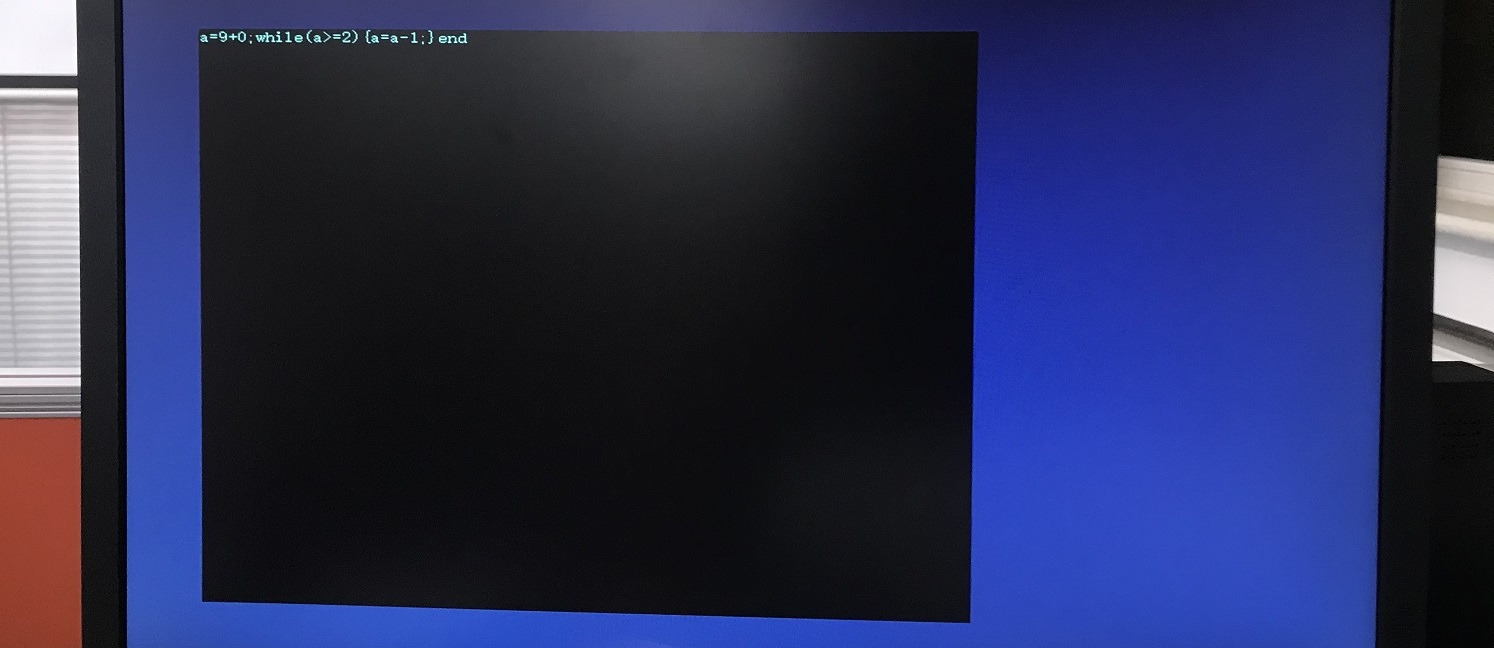
\includegraphics[width=\textwidth]{p01.png}
  \caption{基础界面展示}
\end{figure}

输入功能

\begin{figure}[H]
	\centering
	
\includegraphics[width=\textwidth]{p02.png}
	\caption{输入一些字符、空格和“hello world"}
\end{figure}

退格功能

\begin{figure}[H]
	\centering
	
\includegraphics[width=\textwidth]{p03.png}
	\caption{按退格键前}
\end{figure}


\begin{figure}[H]
	\centering
	
\includegraphics[width=\textwidth]{p04.png}
	\caption{按退格键后}
\end{figure}

\subsection{简单程序执行}

输入简单程序

\begin{figure}[H]
	\centering
	
\includegraphics[width=\textwidth]{p05.png}
	\caption{输入“a=3+3"}
\end{figure}

按动编译按钮,程序尚未执行

\begin{figure}[H]
	\centering
	
\includegraphics[width=\textwidth]{p06.png}
	\caption{按动编译按钮}
\end{figure}

按动执行按钮,程序执行

\begin{figure}[H]
	\centering
	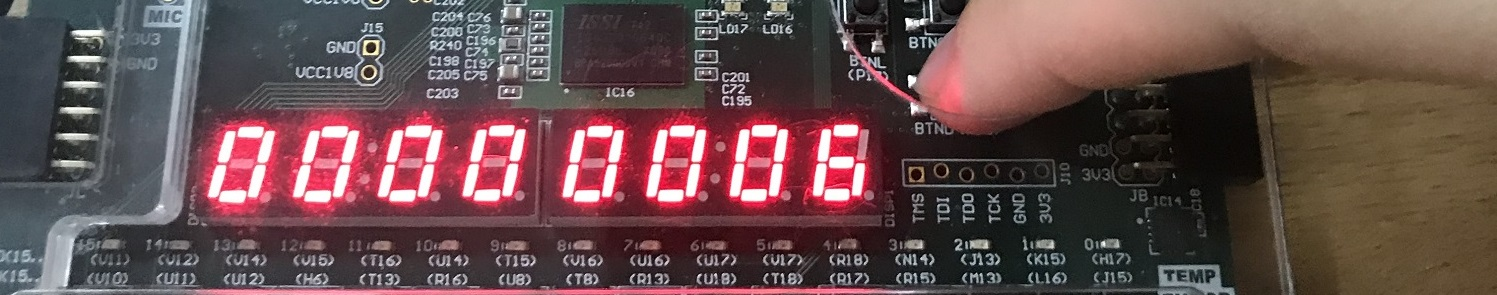
\includegraphics[width=\textwidth]{p07.png}
	\caption{按动执行按钮}
\end{figure}

发现a值变为6,符合代码预期。

\subsection{较复杂代码的编译和执行}

代码如图,带有循环和条件判断结构

\begin{figure}[H]
	\centering
	
\includegraphics[width=\textwidth]{p08.png}
	\caption{复杂的代码}
\end{figure}

按动编译按钮,程序尚未执行

\begin{figure}[H]
	\centering
	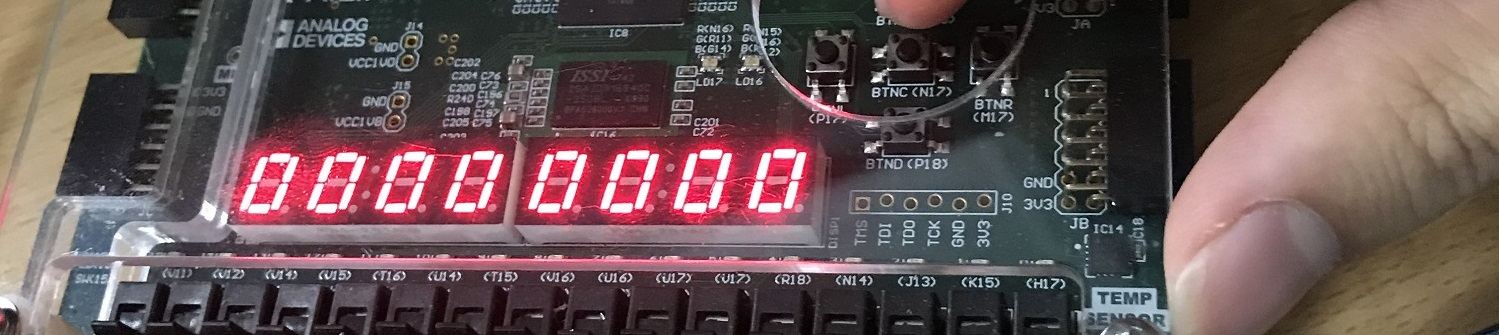
\includegraphics[width=\textwidth]{p09.png}
	\caption{按动编译按钮}
\end{figure}

按动执行按钮,程序执行

\begin{figure}[H]
	\centering
	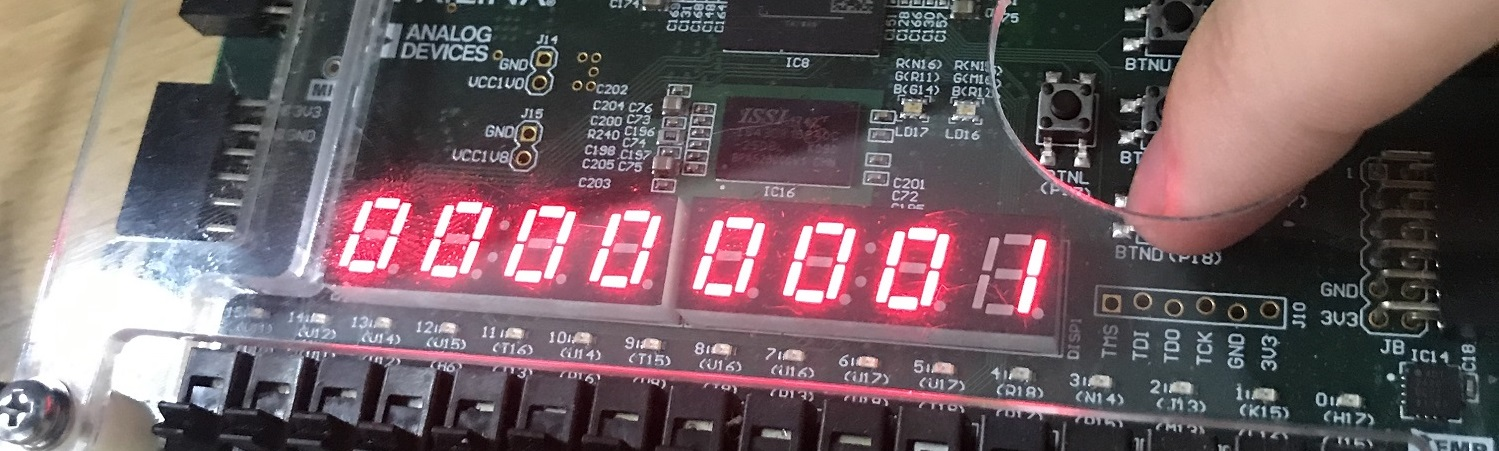
\includegraphics[width=\textwidth]{p10.png}
	\caption{按动执行按钮}
\end{figure}

结果为a=1,符合代码预期,验证通过!

\section{总结的话}
本次综合实验的体验相当难忘。在将来探索的过程中,这次从不可能到可能的经历,或许会成为鼓励我继续走下去的支持之一。

开始便有写编译器的打算,但我并不抱太大完成的希望。在没有任何编译相关知识的帮助下,实验能够成功实在要得益于一开始就想到了Queue队列和使用状态机进行读入的思路。在有了这些思路后,我马上尝试着将整个架构搭建起来。而这些看似过于脑洞的设计,倘若切实试着去做而不是让它就这么躺在设想里,竟真的让我看见了实现编译器的可能。
 
实现设想有个很大的麻烦:设计时的思路往往是顺序执行的,但Verilog作为一种描述性语言,实际书写是要作并行处理看待的。处理这二者间矛盾的办法主要有三个部分,一个是随时钟变化的片选信号,这适用于模块间次序的管理,另一个是局部采用计数器驱动的策略,这适用于细化模块内部某一过程的执行次序,在某些变量赋值与判断语句密集,彼此容易发生冲突的过程中,这是一个有效的分离办法。再一个是针对某个模块具有循环性的过程,通常采用定长的位移状态机作为驱动,利用一个使能信号进行循环开始和结束的控制。

整个实验中最麻烦的部分发生在编译到执行的代码核对上。编译的状态机包含最多96bit的有效信息,而执行程序的每个结点都有64bit位数不均的信息块组合,最后作为实现载体的变量表含有144位的变化信息,从编译到执行,其间包括至少12个步骤需要整合。在缺乏分析工具的时候,每一次Debug都意味着大量的手算和比对。

一方面这让我感觉到如果技术链要达到有效的迭代的话,每个环节都要为后期的分析甚至Debug做些准备,就像编写转COE文件的C程序。如果我需要设计一个功能全面得多的编译器,那么针对这些编码表、状态机、程序结点,势必要先写好相应的分析程序,以免去后期Debug时手动试转译的时间精力。

另一方面,我也学到了一种截然不同的编写风格。作为初学计算机技术者,在编程实习的时候往往喜欢守在键盘前噼里啪啦,其间夹杂着冗长的Debug过程。但在设计这个实验的时候,大部分的时间反倒与电脑无关,而是在草稿纸上仔细推演设计。上机时先出骨架测试,再谨慎地细化。这个做法的直接结果就是写下的代码留存率极高,Debug的次数大大减少,而且即便面临着比往期都要复杂的状态量,我也能很快地看出问题在哪里。实验中采用循环计数器分并行为顺序、上下沿调整等技巧就是那极有限次Debug的直接收获。


%\nocite{*}
%\bibliography{wpref}

\end{document}
